\chapter{Objetivos}
\label{Objetivos}

Los objetivos responden a la pregunta: \textbf{¿Para qué investigar?.} Expresan el resultado que se pretende alcanzar en la investigación, en términos generales y específicos. Han de ser claros, medibles y observables en el tiempo y en el espacio. Un objetivo de investigación consta de dos partes fundamentales: un verbo en infinitivo y la variable a medirse.

En cuanto a su redacción, \cite{herrera2004tutoria} señala que \textit{ “…en los objetivos específicos se emplean verbos que indiquen logros concretos y bien delimitados; por ejemplo comprobar, confirmar, construir, definir, discernir, demostrar, detectar, determinar, describir, discriminar, diseñar, elabora, evaluar, fabricar formula, generar, identificar, locarizar…”.} Conviene anotar que son los objetivos específicos los que se investigan y no el objetivo general, ya que éste se logra en función de los hallazgos de los resultados y la metodología utilizada.

Todo proyecto de investigación es evaluado por el logro de los objetivos. La sistematización hace posible el planeamiento de estrategias válidas para alcanzar los objetivos, éstos tienen que ser revisados en cada una de las etapas del proceso; el no hacerlo puede ocasionar errores. 

\textbf{Al finalizar el proceso, los objetivos han de corresponderse con los resultados.}

Los objetivos de investigación no deben confundirse con las actividades o procesos 
implícitos en el estudio. Ejemplo: Aplicar encuestas y entrevistas a los directivos de la 
Institución educativa XY; motivar al personal de la Organización XY.

No plantear mas 3 de objetivos específicos.

Referencia \url{https://www.youtube.com/watch?v=pNgwVGy0d6A}

\section{General}
Aquí el objetivo general en español.

Put the project targets


\section{Específicos}
\begin{itemize}
    \item Objetivo específico 1
    \item Objetivo específico 2
    \item Objetivo específico 3
\end{itemize}


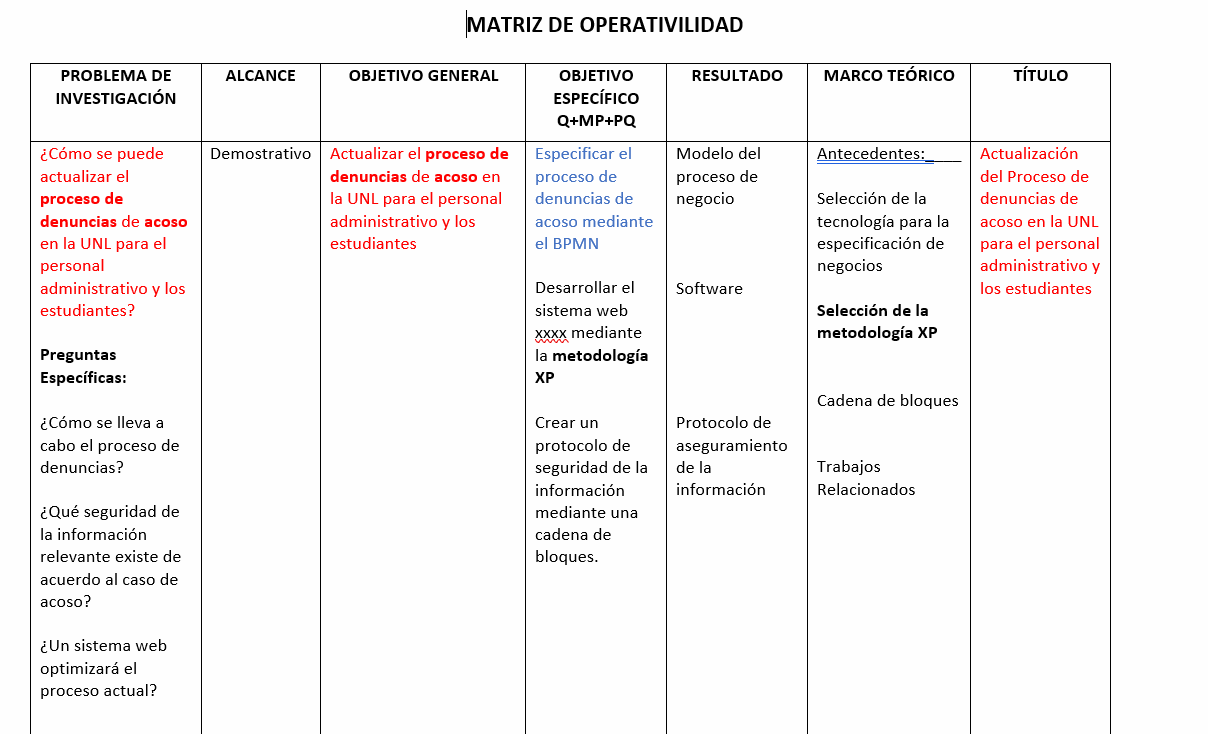
\includegraphics[scale=0.6]{img/matriz.png}